We follow the usual VOF method and will only detail the necessary steps to illustrate the momentum advection method based on the VOF method in the next section. Moreover we will use in this section a rescaling of the space and time variables so that the cell size is 1, and the time step is also 1. All velocities are then rescaled to $u^\prime = u \tau / h$. Because of this space rescaling and in these new units, $\cijk$ is also the measure of the volume of reference fluid in cell $i,j,k$.


\subsubsection{Volume initialisation}

Before any VOF interface tracking is performed, the field of $\cijk$
values must be initialized. We use the {\sc Vofi} library described in \cite{bna2015numerical} and \cite{bna2016vofi}. 
This allows a high-accuracy numerical integration of the measure of the fluid volumes. 

\subsubsection{Normal vector determination} 

The VOF method proceeds in two steps, reconstruction and advection. In
the reconstruction step, one attempts to obtain the ``best'' possible representation of the interface 
using Volume of Fluid data $\cijk$. The best representation is usually the one with the smallest 
reconstruction error for objects such as circles or ellipses, but issues of continuity and robustness 
at low resolution may also be considered. In the work reported here 
we use a standard method  described in \cite{Tryggvason11}.  In each cell cut by the interface
one first determines the interface normal
vector $\N$, then one solves the problem of finding a plane perpendicular
to $\N$ under which one finds exactly the volume $\cijk$. Normal vector determination
is performed using the MYC method described in \cite{Tryggvason11}. 

\subsubsection{Plane constant determination}

Once the interface normal vector $\N$ is determined, a new,
colinear normal vector noted $\M$ and having unit $L_1$ norm is
deduced from $\N$, so that $|m_x| + |m_y| + |m_z|=1$. Considering the
volume $V=\cijk$ in cell $i,j,k$ the plane constant $\alpha$ is
defined so that the plane 
\be 
\M \cdot \X = \alpha \label{mxalpha}
\nd 
cuts exactly a volume $V$ in the cell.   
Typically $\alpha$ is determined by the resolution of a cubic equation as described
in \cite{Scardovelli00}.

\subsubsection{General split-direction advection}
\label{generalsplit}
Once the reconstruction has been performed at time $t_{n}$, it is used to obtain the approximate position of the interface, and the volumes $\cijk$ at time $t_{n+1}$. The following discussion of momentum advection is based on 
two VOF advection methods, (Figure \ref{lagfig})  Lagrangian Explicit
and  Weymouth and Yue advection. We first describe the common features of these two methods. 

After addition and subtraction of a term proportional to the velocity divergence, 
equation (\ref{interfadv}) leads to 
\be
\dert H + \nabla \cdot (\U H) = H\, \nabla \cdot \U \,.
\nd
A discrete representation of this equation is obtained by integrating the advection equation 
in time and space
\be
{\cijk^{n+1} - \cijk^{n}} = - \sum_{\rm{faces}\, f} F^{(c)}_f + \int_{t_n}^{t_{n+1}}  
{\rm d}t \int_\Omega  H \,\nabla \cdot \U\,  {\rm d}\X   \,,
\label{sumf}
\nd
where the first term on the right-hand side is the sum over faces $f$ of cell $i,j,k$ 
of the fluxes $F^{(c)}_f$ of $\U H$. Obviously the ``compression'' term on the right-hand side 
disappears for incompressible flow, however it is useful to keep it in view of its utility 
in split-advection methods.  In the previous equation $F_f^{(c)}$ is defined by
\be
F_f^{(c)} = \int_{t_n}^{t_{n+1}} {\rm d}t \int_{f} u_f(\X,t) H(\X,t) \, {\rm d}\X \,,
\label{faceint}
\nd
where $u_f = \U\cdot \N_f$ and $\N_f$ is the unit normal vector of face $f$, pointing outwards of cell $i,j,k$. 

Once an approximation for the evolution of $\U(\X,t) H(\X,t)$ during
the time step is chosen, a four-dimensional integral remains to be
computed in equation (\ref{faceint}). In what follows we describe the
approximations used. However, all the methods we describe here
are directionally split. The methods are also designed to preserve the
property that $0 \le \cijk \le 1$ which we call $C$-bracketing. It
is important to preserve $C$-bracketing despite the various
approximations used, in order to avoid the arbitrary addition or
removal of mass.

Directional splitting results in the breakdown of equation (\ref{sumf}) 
into three equations
\be
{\cijk^{n,m+1} - \cijk^{n,m}} = - F^{(c)}_{m-} - F^{(c)}_{m+} 
+ c_m \partial_{m}^h u_m \,,
\label{sumf2}
\nd
where $m=1,2,3$, $\cijk^{n,1} = \cijk^{n}$,  $\cijk^{n,4} = \cijk^{n+1}$, the face 
labelled ``$m-$'' is the ``left'' face in direction $m$ with $F^{(c)}_{m-} \ge 0$
if the flow is locally from ``right'' to ``left'', and finally the face ``$m+$'' is the 
``right'' face in direction $m$ with $F^{(c)}_{m+} \ge 0$ if the flow is from ``left'' 
to ``right''. We have also  approximated the compression term in 
(\ref{sumf}) by
\be
 \int_{t_n}^{t_{n+1}}  {\rm d}t \int_\Omega  H \partial_m u_m  {\rm d}\X \simeq  c_m 
 \partial_{m}^h u_m \,, 
 \label{comp}
\nd
with no implicit summation rule. 
 In the RHS of (\ref{sumf2}) and \ref{comp}) the flux terms $F_{f}^{(c)}$ and the 
 partial derivative $\partial_{m} u_m$ must
be evaluated with the same discretized velocities. In particular,
$\partial_{m}^h u_m$ is a finite difference or finite volume approximation of the 
spatial derivative of the $m$th component of the velocity vector in direction $m$, and
the ``compression coefficient'' $c_m$ approximates the color fraction. Its exact expression 
is dependent on the version of the directionally 
split advection method used and will be described below. 
The value of $c_m$ is chosen so as to preserve the $C$-bracketing condition. 
Note that because $c_m$ may not be the same coefficient along the three Cartesian directions,
even if the flow is incompressible the sum $\sum_m c_m \partial_{m}^h u_m$ of the 
split compression terms is not necessarily vanishing.

Each application of 
equation (\ref{sumf2}) defines an advection substep. 
After each substep, a new  reconstruction of the interface is performed
with the updated volumes $\cijk^{n,m+1}$, 
computing the normal $\M$ and the $\alpha$ constant. This reconstruction is used to estimate the 
fluxes $F^{(c)}_{f}$ in the next split advection substep  (\ref{sumf2}). 

\subsubsection{Lagrangian Explicit advection}

 The Lagrangian Explicit / Calcul d'Interface Affine par Morceaux
CIAM advection method is described in what follows. ``Calcul d'Interface Affine
par Morceaux'' is French for ``Piecewise Linear Interface
Calculation'' (PLIC) but while PLIC refers to a generic VOF method with
a piecewise linear reconstruction step, CIAM refers to a specific type
of advection method first described in the archival literature in
\cite{li95} and classified as the ``LE'' method in
\cite{Scardovelli02}.  CIAM advection is most naturally explained
as a Lagrangian transport of the Heaviside function. In each cell, the
reconstruction step has defined a planar interface. Lagrangian
transport consists in moving each point of this interface by
a velocity field $\U'$ defined as follows: 1) in each sub time step
$m$ of split advection the velocity field is in direction $m$, and
depends only on the component $x_m$ of the space variable; 2) the
velocity field is interpolated between the face velocities $u_{m-}$ on
the left face and $u_{m+}$ on the right face so that 
$u_m' ( x_m) = - u_{m-}( 1 - x_m) + u_{m+} x_m$ where the origin of the coordinate
$x_m$ was chosen on the left face. (As said before, space has been
rescaled so the cell size is unity and recall $u_f = \U\cdot \N_f$.) 
The exact transport by this velocity field is $d x_m / dt = u_m'(x_m)$ but we use 
a first-order, explicit approximation as $x_m^{n+1} - x_m^n = u_m'(x_m^n)$. 
(Time was rescaled so the time step is unity and disappears from the equations.) 
Using the approximation for the interpolated velocity we get 
\be
x_m^{n+1} =  - u_{m-} +  (1 +  u_{m+} + u_{m-}) \,x^n_m \,.
\label{map}
\nd
This relation gives the
advected points of the interface as a function of the original
points. It is used to advect the faces and the planar interfaces as
shown on Figure \ref{macfig}, for a two-dimensional case. After advection, at most 
three interface fragments are found in each cell. The resulting volumes 
(areas in 2D) are shown in Figure \ref{lagfig} and are labelled $V_1$, $V_2$ and $V_3$. 
Eventually 
\begin{figure}
\begin{center}
    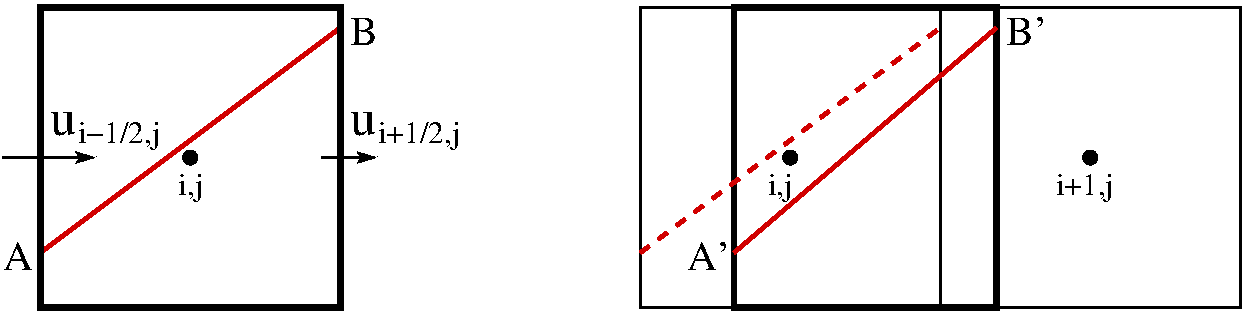
\includegraphics[width=0.75 \textwidth]{Figures/band1bis}
\end{center}
\caption{Advection of the AB interface segment. Face velocities at the left face, 
$u_{i-1/2,j} = -u_{1-}$, and the right face, $u_{i+1/2,j} = u_{1+}$,
are used to create an interpolated linear velocity field, so that point $A$ is advected 
to point $A'$ at the velocity $u_{i-1/2,j}$, point $B$ to $B'$ at  the velocity $u_{i+1/2,j}$, 
and a point along AB at a velocity linearly interpolated between $u_{i-1/2,j}$ and  $u_{i+1/2,j}$.}
\label{macfig}
\end{figure}
\begin{figure}
\begin{center}
    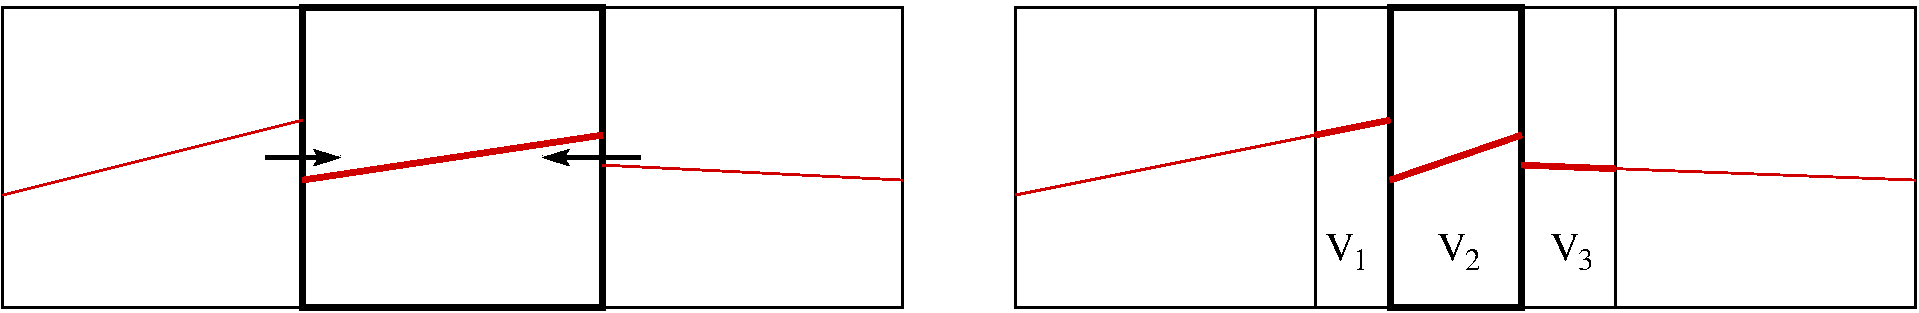
\includegraphics[width=\textwidth]{Figures/LE_mapping-horbis.pdf}
\end{center}
\caption{Formation of the volumes  $V_1,V_2$ and $V_3$ by Lagrangian advection in the $x$ direction. 
Left: initial reconstruction with the horizontal velocities on the faces of the central cell. 
Right: segments and volumes $V_i$ (see text) after Lagrangian advection (for simplicity it has been 
assumed $u_{i-3/2,j} = u_{i+3/2,j} = 0$)}
\label{lagfig}
\end{figure}
the color function is given by the sum of three contributions
\be
\cijk^{n,m+1} =  V_1 + V_2 + V_3 \,.
\nd
It is seen that the transform (\ref{map}) compresses distances by a factor 
$1 + \partial^h_m u_m = 1 + u_{m+} +  u_{m-}$. 
Thus the measure of any region of space is scaled by this amount under advection. 
The interface is then transfomed in three steps: 
1) compress all cells by the factor above; 
2) move the cells by $u_{m-}$; 
3) the moved cells now overlap the original cells. 
The volume corresponding to the overlap of the cell with itself is $V_2$, 
while $V_1$ and $V_3$ correspond
to the overlap with the moved cells from the left and right, respectively. 
The geometrical interpretation of the Lagrangian Explicit advection 
of Figs. \ref{macfig} and \ref{lagfig} and the definition
\eqref{faceint} of $F^{(c)}_{f}$ \blue{ leads to the following correspondence between 
the fluxes and the volume contributions $V_i$. 
To start with an example, for the central cell of Fig. \ref{lagfig} the flux on
the left face is from left to right, since $u_{1-} = - u_{i-1/2,j} < 0$.
This means that $V_1 =  - F^{(c)}_{1-,i} =  F^{(c)}_{1+,i-1} > 0$ while $V_3$ of the left cell, that
is $V_{3,i-1}$, is zero corresponding to an absence in that cell.
In all cases the fluxes accross a face are equal to the 
$V_1$ or $V_3$ of one cell or the other adjacent
to a face. }
The final expression of the split step is then
\be
\cijk^{n,m+1} =  \cijk^{n,m} (1  +  u_{m+} +  u_{m-} )  - F^{(c)}_{m-} - F^{(c)}_{m+} \,,
\label{sumflag}
\nd
which shows that the constant $c_m$ in the compression term is $\cijk^{n,m}$ while the 
approximation of the derivative is $\partial_m^h u_m =u_{m+}  + u_{m-} $ . 

It is interesting to note that using three Lagrangian advections in a sequence does not result in 
volume conservation to machine accuracy. Indeed the summation of the three substeps (\ref{sumf2}) 
results in 
\be
{\cijk^{n+1} - \cijk^{n}} = - \sum_{\rm{faces}\, f} F^{(c)}_f 
+ \sum_{m=1}^{3} \cijk^{n,m}(u_{m+}  + u_{m-}) \,.
\label{sumfall}
\nd
While the flux terms cancel upon integration over the domain, the sum of the compressive terms 
does not vanish since $\cijk^{n,m}$ changes during the three substeps.
We recover eq. \refeq{sumf2} with 
\be
c_m = \cijk^{n,m} \label{cmle}
\nd
\begin{figure}
\begin{center}
    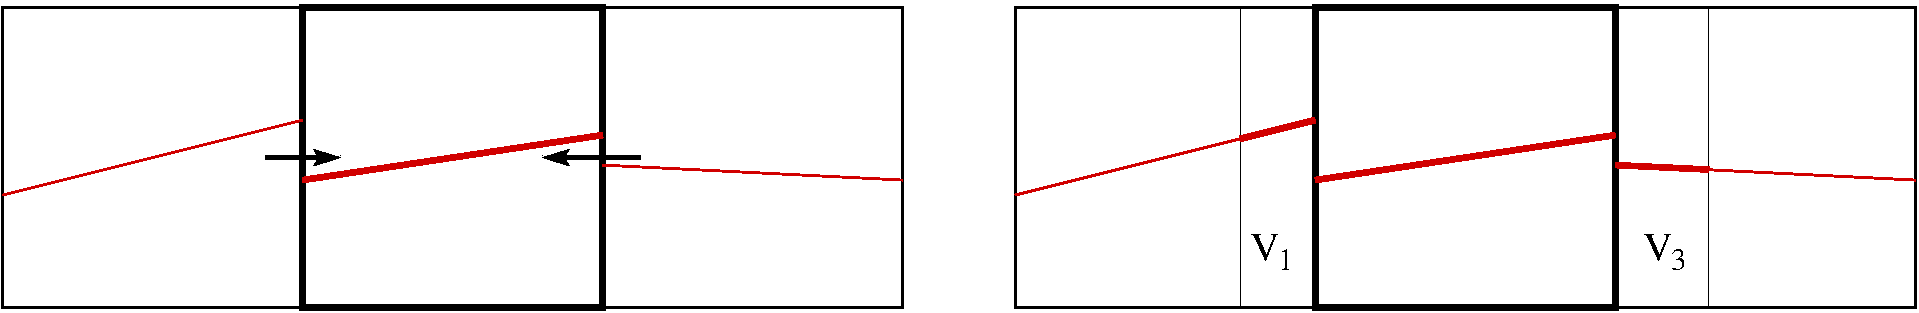
\includegraphics[width=\textwidth]{Figures/EI_mapping-horbis}
\end{center}
\caption{Eulerian flux representation for advection in the $x$ direction. 
Left: same initial reconstruction of Fig. \ref{lagfig} with the horizontal velocities 
on the faces of the central cell. 
Right: fluxes, or volumes $V_1$ and $V_3$, are calculated directly from the interface
reconstruction in each cell}
\label{eulflux}
\end{figure}

\subsubsection{Weymouth and Yue advection}

Another method that we shall describe is the exactly mass-conserving method of Weymouth and Yue (WY) 
described in ref. \cite{Weymouth:2010hy}. In that method the coefficient of the compression term  
(\ref{comp})
is independent of the direction $m$ so that $c_m = c$. The coefficient $c$ is defined as
\be
c=\Theta(\cijk^n - 1/2) \label{cmwy}
\nd
where $\Theta$ is the one-dimensional Heaviside function (defined on the real axis). 
That is $c=0$ if $\cijk^n < 1/2$ and $c=1$ if  $\cijk^n \ge 1/2$. 
The fluxes $F^{(c)}_f$ are also defined differently. The left fluxed volume in direction $m=1$ 
is equal to the volume fraction $F_{1-}^{(c)}$ in a cuboid of width $u_{i-1/2,j,k}$ 
(recall that $\tau = 1$) adjacent to the left face $f=1-$. This fluxed volume corresponds to 
``Eulerian Implicit'' (EI) advection in the terminology of \cite{Scardovelli02}
and is represented by the volume $V_1$ on Figure \ref{eulflux}. Using these definitions,  
Weymouth and Yue were able to show in ref. \cite{Weymouth:2010hy} that the final result obeys 
$C$-bracketing (see Section \ref{generalsplit}). 

Using  this advection method  results in volume conservation at machine accuracy. 
Indeed the summation of the three substeps (\ref{sumf2}) results in 
\be
{\cijk^{n+1} - \cijk^{n}} = - \sum_{\rm{faces}\, f} F^{(c)}_f 
+ c \sum_{m=1}^{3} \partial_{m}^h u_m \label{sumfall2}
\nd
Since $\sum_{m=1}^{3} \partial_{m}^h u_m = \sum_{m=1}^{3} (u_{m+}  + u_{m-}) $ is the simple 
finite-volume expression for $\nabla \cdot \U$, it disappears and mass is conserved at the 
accuracy with which condition (\ref{divu}) is satisfied. 

\subsubsection{Clipping}
\label{clipping}

The algorithm that has been coded involves a number of additional
steps designed to avoid unwanted effects of arithmetic floating point
round-off error. The most important one is clipping: at the end of
each directional advection, the values of $\cijk$ are reset so that
$C_{ijk}$ is set to $0$ is $C_{ijk} < \eps_c$ and $C_{ijk}$ is set to
$1$ is $C_{ijk} > 1 - \eps_c$. When there is no surface tension 
%with large curvature $\kappa h$ 
the choice $\eps_c = 10^{-12}$ works well.
Otherwise $\eps_c = 10^{-8}$ gives more stable results with smoother
interface shapes. This stronger clipping is a necessity for some
simulations with WY, while the CIAM method can survive $\eps_c =
10^{-12}$ with the diffusive interpolation schemes described below.  
As a matter of fact we observe that WY produces many more ``wisps'', 
i.e. cells with tiny values of $1-\cijk$
inside the liquid or $\cijk$ inside the gas.
We have not yet been able to determine the origin of this need for a more
forceful clipping with WY, but it could be related to the fact that the
CIAM method has a geometrical interpretation, while WY is intrisically algebraic
in nature.
